%%% Results %%%
\chapter{Results \& Evaluation} \label{ch:results}
This chapter presents the evaluation criteria for the endorsement model
proposed in chapter ~\ref{ch:method}. Based on which, the overall system design
and functionality will be evaluated and final results is presented. 

\section{Evaluation Criteria}
To assess the fulfillment of requirements, a descriptive approach based on the
design evaluation method by Hevner A, Chatterjee S.~\cite{hevner2010design} is
used when necessary. The system is not only reliant on the smart contract code
and its execution but also on the interaction theory discussed. For this, the
endorsement interaction is simulated using the graph simulation tool
ne04j~\footnote{https://neo4j.com/}. The dataset used to simulate the
interaction is taken from SNAP~\cite{snapnets}. The details on the dataset are
presented in Section~\ref{sec:interaction}. Given the time constraints, no form of
structural/unit testing was performed. The purpose of this project was a PoC
design to demonstrate the reputation model as a use case via the use of smart
contracts and blockchain technology. An extensive experiment to simulate a
real-world usage was not performed. However, manual testing was done during
development using ganache~\footnote{https://github.com/trufflesuite/ganache}
and deployment of contract on a local network. Additionally, front-end was
developed to test contract function calls and communicate with contracts on
blockchain network from the browser itself. 

\section{Fulfillment of User stories and Requirements}\label{fulfillment}
The method to examine fulfillment of user stories and requirement follows the
method used by Hevner's descriptive design evaluation
approach~\cite{hevner2010design}. The table~\ref{table:fulfillment} presents
the motivation for fulfillment of functional requirements. For the relevant
smart contract code, refer to the appendix~\ref{smartcontracts}. 
The fulfillment of non-functional system requirements is discussed below:
\paragraph{Smart contract security:}The security considerations by
Solidity~\cite{soliditySecurity} was followed for the contract code. Not all
the recommendations presented there were relevant for the endorsement contract.
For instance, recommendations on restricting the amount of ether or patterns
for sending/receiving ether in a function call is not relevant as endorsement
contract does not require any function call to include any amount of ether as
the message value. As part of fail-early principle, the contract function code
was ordered as conditions, actions, and interactions where relevant. Doing so
can avoid Re-Entrancy bug. The function call can be made by both externally
owned account or a contract address in ethereum. A maliciously crafted contract
can make a function call repeatedly before the execution of the function ends
or throws an exception which can cause the function to interact in unintended
ways. As such, failing early by making the checks first in a function can avoid
such bugs. 
\begin{center} \label{table:fulfillment} 
	\begin{table}
		\begin{tabular} {| l | l | p{9cm} | }
		\hline
		\textbf{User}  & \textbf{Traceability}   & \textbf{Motivation for fulfillment} \\
		\hline
		\multirow{2}{*}{Endorser} & R1 & Any registered participant can make a
		call to endorse() function to send an endorsement to other registered
		participants on the network.      
		\\\cline{2-3} 
		& R2  & Any registered participant can call removeEndorsement()
		function just by providing the address of the endorsee they wish to
		remove.  \\\cline{2-3}
		& R3 & Each call to endorse() function updates the state variable of
		the current endorser and endorsee, storing and updating the respective
		state variables. i.e., nEG, nER, index. This function call also invokes
		updateEndorsee() function to update the endorsee information
		accordingly.  \\\cline{2-3}
		\hline
		\multirow{2}{*}{Endorsee} & R5.& The storage of personal information
		was not fully implemented by the endorsement PoC, therefore, editing
		personal information is irrelevant. However, change to pseudonym can be
		possible by just making a call to editProfile() by the participant.
		\\\cline{2-3}
		\hline
		\multirow{2}{*}{other users} & R4.1 & Anyone can make a call to
		computeImpact() function to get the final computed score of a
		participant based on public key hash registered on the endorsement
		network. \\\cline{2-3}
		& R4.2 &  Anyone can make a call to joinNetwork() function and become a
		registered participant of the network immediately.  \\\cline{2-3}
		\hline
	\end{tabular}
	\caption{Fulfillment of User stories and Requirements for Endorsement PoC}
\end{table}
\end{center}
%\begin{lstlisting}[language=Solidity]
%	function joinNetwork(string _userName) public{
%		//conditions: only allow unregistered participant
%		require(!joined[msg.sender]);
%
%		//actions
%		joined[msg.sender] = true;
%		
%        //Interaction
%		Participant memory newParticipant = Participant({
%				identifier: msg.sender,
%				name: _userName
%        });
%		participants.push(newParticipant);
%        LogJoinNetwork(msg.sender, _userName);
%        numberOfParticipants++;
%        participantIndex[msg.sender] = numberOfParticipants-1;
%    }
%\end{lstlisting}
\vspace{-15mm}
\paragraph{Reliability:}This requirement relates to the immutability of data
stored on the blockchain network which is ensured by \ac{PoW} consensus
algorithm. The data is stored on a public, permission less blockchain network
which allows any node to commit a block of transactions to the blockchain. A
validator node collates the list of transactions into a block. A malicious node
that intends to double spend a transaction can do so by solving the
cryptographic puzzle in parallel with the rest of the network. If the malicious
does not broadcast the solved blocks to the network and instead keeps solving
the puzzle in isolation with the network. The transactions that the malicious
node spent can be included in the blockchain that the network is in agreement
with currently. After a certain length of blocks has been solved, the malicious
node can then decide to broadcast his version of blockchain to the network.
Blockchain protocol ensures that the network switches to the longest chain in
the event of a fork. Since the malicious node is in a race with the rest of the
network, this form of attack is only possible if the malicious node owns more
than 51\% of the hashing power compared to the rest of the network. Therefore,
this attack is called 51\% attack. As long as honest nodes control half of the
network, the \ac{PoW} mechanism ensures an immutable record of transactions to
be stored in the blockchain.

\paragraph{Trust metrics correctly describe the actual trust of the nodes:}The
fulfillment of this requirement is assessed by simulating an interaction graph
and analyzing different scenarios in the network. The
Section~\ref{sec:interaction} presents the details regarding this requirement. 
%%%%%%%%%%%%%%%%%%%%%%%%%%%%%%%%%%%%%%%%%%%%%%%%%%%%%%%%%%%%%%%
\section{Interaction graph} \label{sec:interaction}
For the simulation of user interaction in endorsement network and the resulting
impact value, a real-world data set was used. The dataset was extracted from
Bitcoin Alpha trust~\footnote{https://alphabtc.com/blockchain/} weighted signed
network which is a who-trusts-whom network of people that trade on Bitcoin
Alpha platform. Participants on this network rated each other on a scale of -10
to +10 where negative value represented total distrust whereas positive value
represented total trust. It consisted of 3,783 nodes that made 24,186 edges out
of which 93\% of the edges were marked as positive edges\cite{kumar2016edge}.
The available information in the dataset for all the nodes was source, target,
rating, and timestamp. All of which is essential information for endorsement
network.
\begin{figure}
	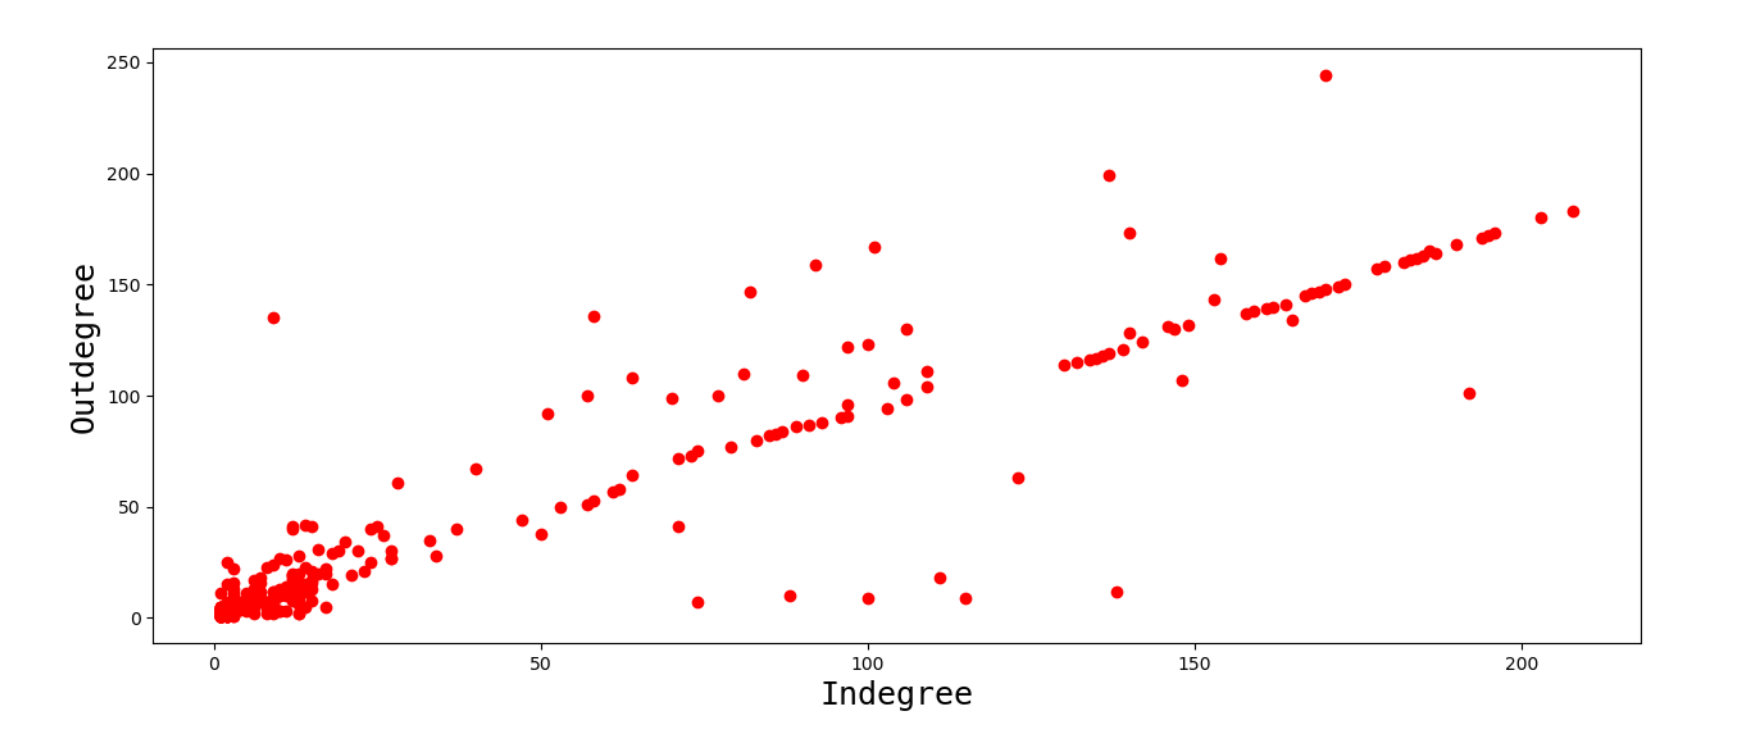
\includegraphics[width=0.95\textwidth]{Images/in_out.eps} 
	\caption{Given Vs. Received} 
	\label{inOut}
\end{figure}
The direction of endorsement is based on the source and target information.
The timestamp information can help to decide on the order of transaction
occurrence in the network. This information is particularly interesting for
anomaly detection algorithm such as Net flow rate convergence as discussed in
\cite{buechler2015decentralized}.  Unlike the Bitcoin Alpha network that let
users rate on a scale of -10 to +10 to demonstrate the strength of their trust
towards other users. The endorsement is more of a boolean decision problem,
i.e., a user either endorses a specific claim made by the entity or does not
endorse. There is no range of values to depict the strength or weakness. For
making it a bit more relevant to endorsement interaction, the existing dataset
was filtered only to have edges with a rating above +2. No negative edges were
considered for the endorsement simulation.  As a result, the total number of
nodes was reduced to 1677 with 4776 edges. Endorsement model was then applied
to these nodes, and their total endorsement impact was computed based on their
incoming and outgoing connections. 
%The scores along with new findings are presented below: 

\paragraph{Total Endorsement Impact:}This value is based on the degree of
connections and ~\ac{TRP} for each node. 70\% (1175 nodes) turned out to have a
\ac{TEI} score of zero. On examining the nodes, they were found to have only
one incoming or outgoing connections. As such, the \ac{TEI} score of zero was
expected because a node would only be considered for making an impact on the
endorsement system if the number of connections is more than one. The score of
zero, in this case, is not representative of a non-trustworthy node, but a
starting node. Thus, we can say that 70\% of the nodes in the network are new
users. This computation leaves us with only 502 nodes to account for having a
considerable \ac{TEI} score. The distribution of \ac{nEG} and \ac{nER} among
the participants of the network is given by Figure~\ref{inOut}. 
\begin{figure}
	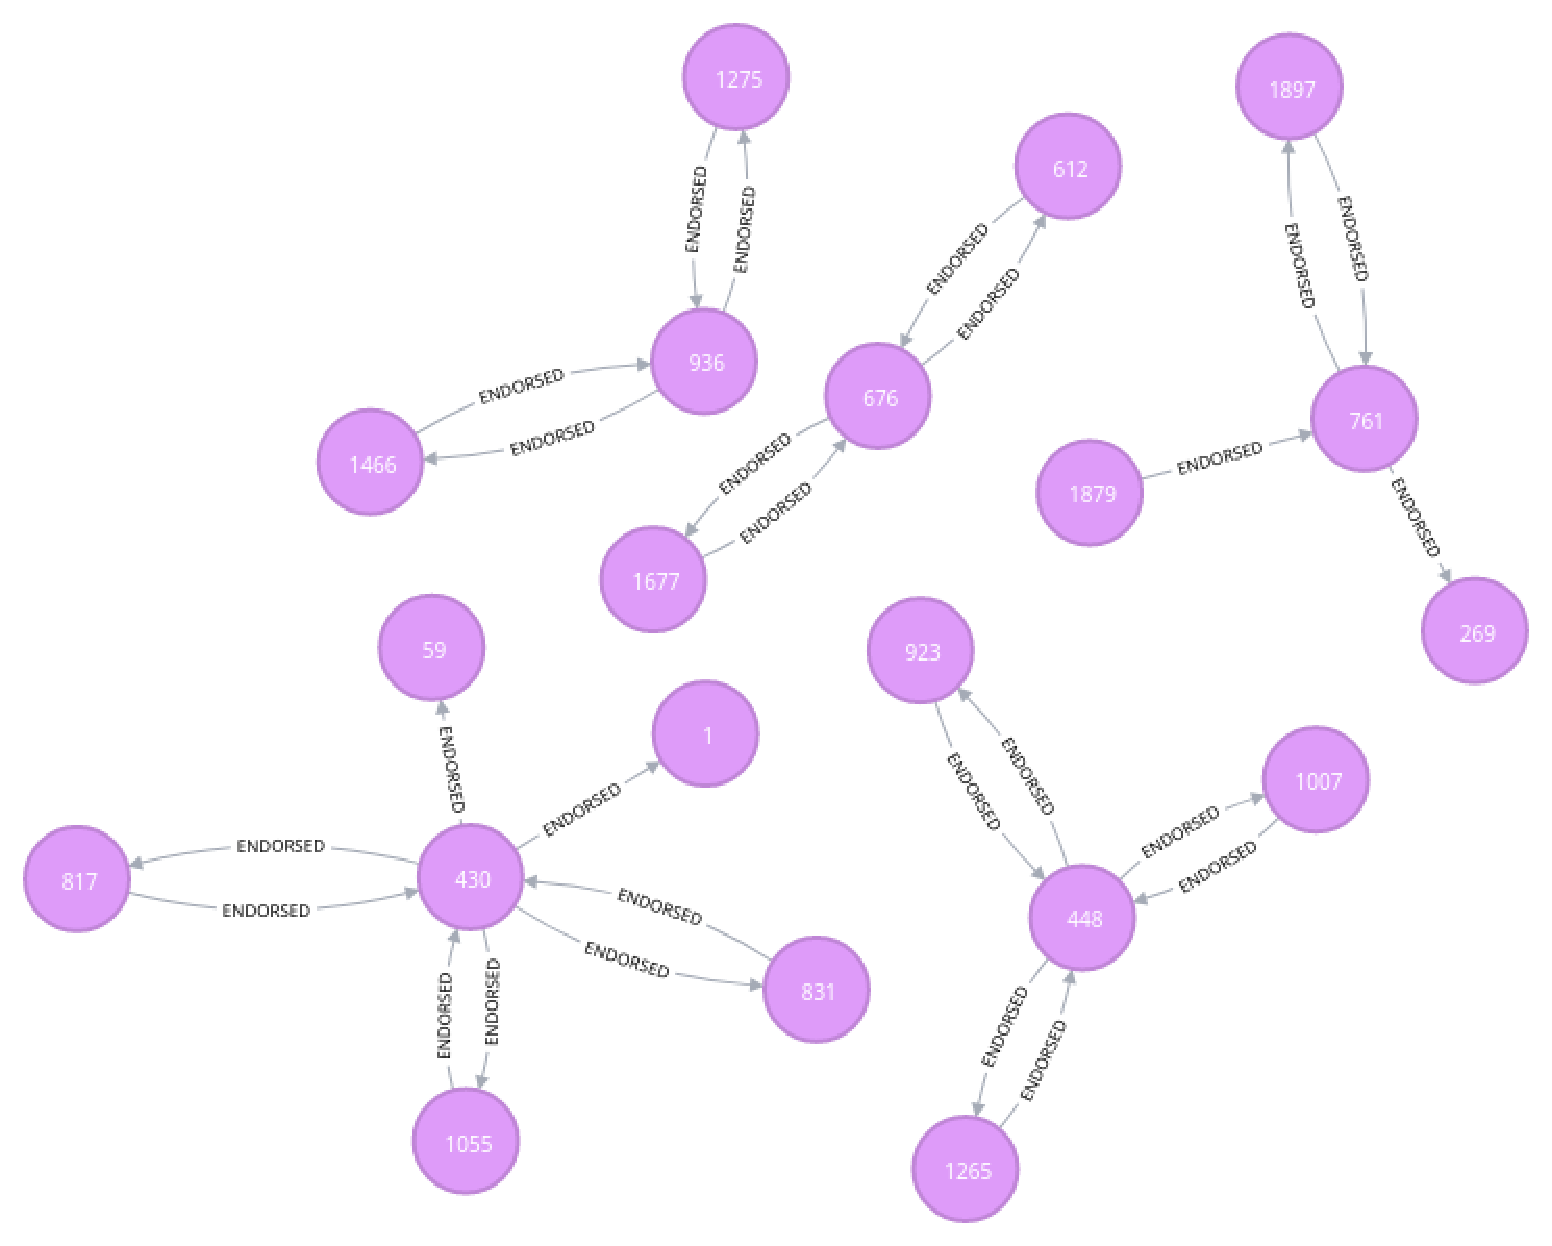
\includegraphics[width=0.95\textwidth]{Images/nodesWithImpactZero.eps}
	\caption{Interaction subgraph of nodes with impact zero}
	\label{fig:zeroimpact}
\end{figure}
\paragraph{Total Received Points:} Among the remaining 502 nodes, there were 5
participants whose \ac{TEI} score was zero despite having more than one
incoming/outgoing connections. This value was because of \ac{TRP}, which is
another significant factor that the endorsement system takes into account.
Though the nodes received endorsements to have a considerable amount of
~\ac{nER}, their \ac{TRP} was zero because the endorsers were not impactful in
the network. The interaction subgraph for these five nodes is shown in
Figure~\ref{fig:zeroimpact}. This factor corresponds to the prestige centrality
metrics of a graph network where the significance of its adjacent nodes
determines the significance of a node. In this case, the significance of a node
is not directly associated with ~\ac{TEI} of the endorser but the value of
\ac{CP} of each endorser that accumulatively contributes to ~\ac{TRP}. The
\ac{CP} of the endorsers for these nodes can be seen in
Figure~\ref{fig:zeroimpact}. The table~\ref{table:receivedpoints} shows the
value for each relevant variables required to compute ~\ac{TEI} for the nodes.
\begin{center} \label{table:receivedpoints}
\begin{tabularx}{\textwidth}{| X | X | X | X | X | X |} 
  \hline
  \textbf{Node label} & \textbf{nEG} & \textbf{nER} & \textbf{ratio} & \textbf{TRP} & \textbf{TEI} \\
  \hline 
  430  & 5 & 3 & 0.6 & 0 & 0  \\
  \hline
   761 & 2 & 2 & 1 & 0 & 0 \\
  \hline
  448 & 3 & 3 & 1 & 0 & 0 \\
  \hline
  676 & 2 & 2 & 1 & 0 & 0 \\
  \hline
  936 & 2 & 2 & 1 & 0 & 0 \\
  \hline
  \caption{Nodes with zero impact and maximum ratio}
 % \label{table:receivedpoints}
\end{tabularx}
\end{center}
%\begin{figure}
%	\includegraphics[width=1.0\textwidth]{Images/TRPVsTEIFontSize.eps}
%	\caption{TRP vs. Total EDS Point}
%	\label{fig:receivedpointsvsimpact}
%\end{figure}

%\begin{figure}
%	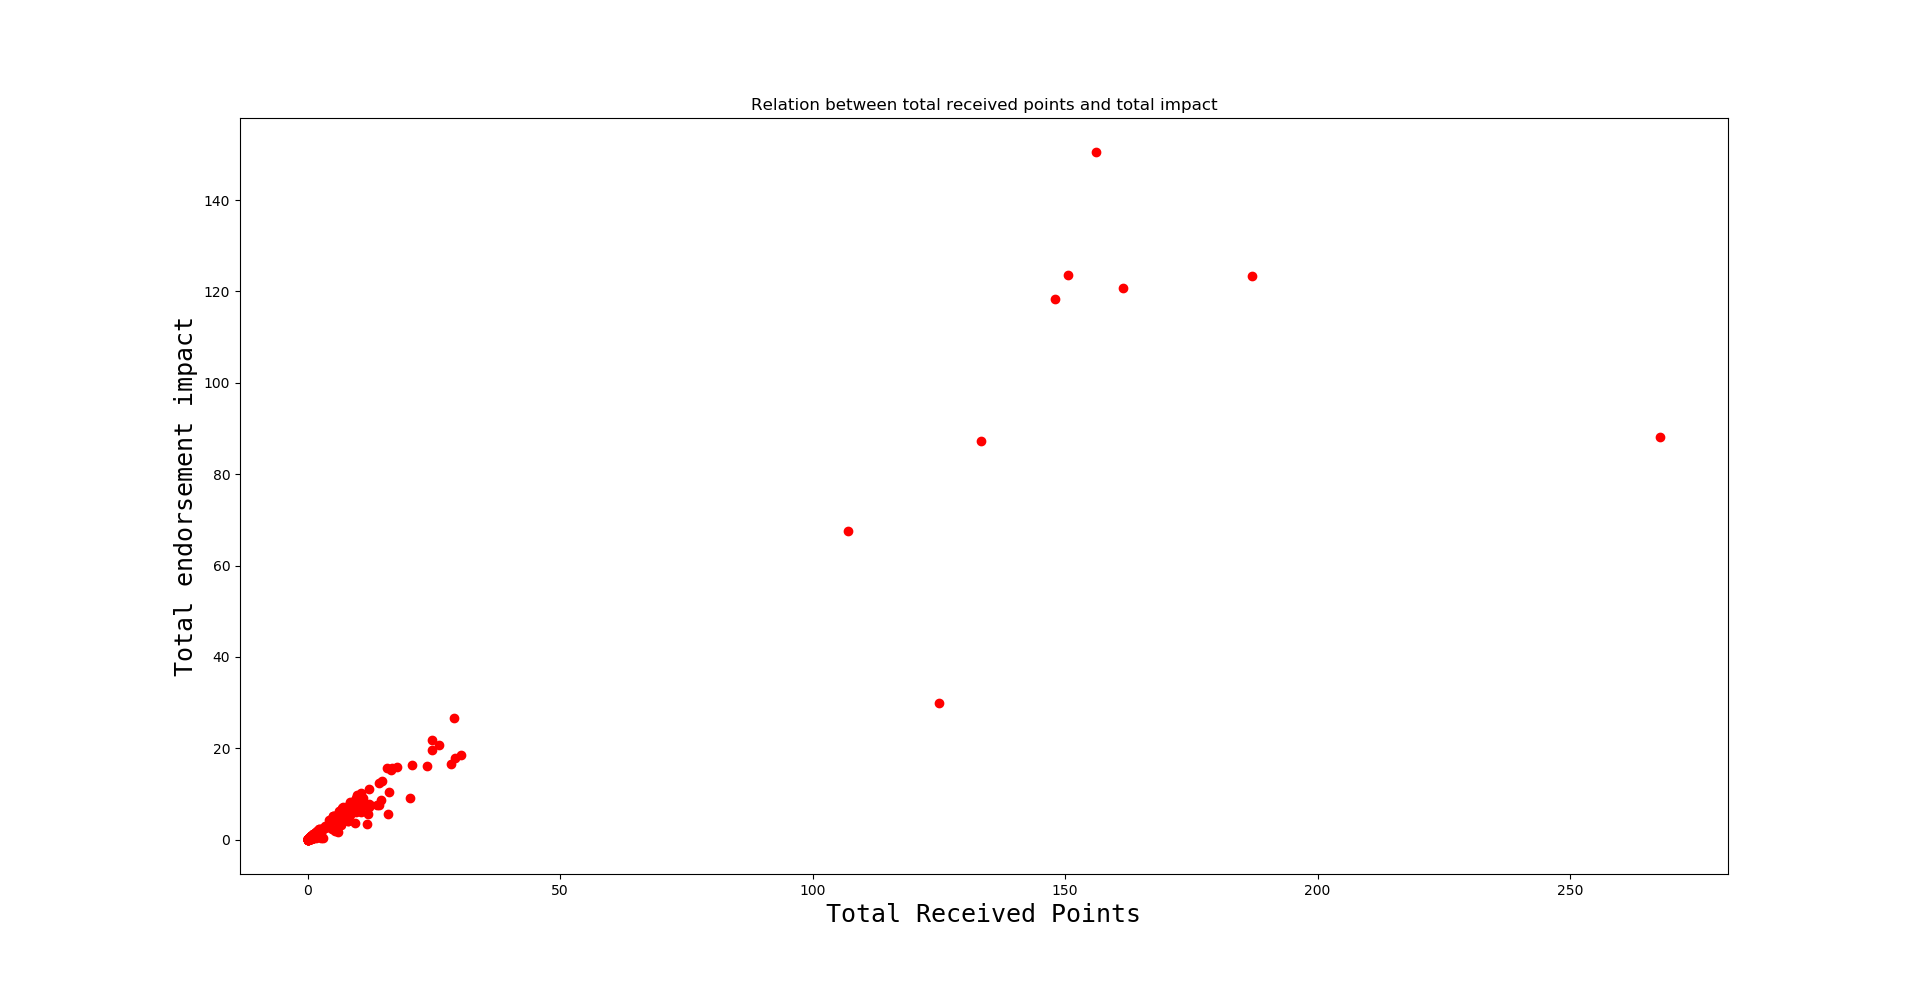
\includegraphics[width=1.0\textwidth]{Images/receivedPoints_impact_impactAboveZero.eps}
%	\caption{Received Points Vs. Total Endorsement Impact}
%	\label{fig:receivedpointvsimpact}
%\end{figure}
\vspace{-15mm}
\paragraph{Ratio:} The information presented by
table~\ref{table:receivedpoints} shows nodes that have the maximum possible
value for ratio which is 1 and still have the lowest \ac{TEI} score. It shows
that maintaining the ratio between outgoing and incoming connections is not
enough to have a significant impact on the network. The
Figure~\ref{fig:ratioimpact} shows the relation between ratio and total
endorsement over all nodes. Based on this relation, we can say that higher
ratio does not mean a higher impact but a higher impact should have a higher
(maintained balance) ratio. Thus, the ratio is a contributing factor to
maintain a significant score in the long run. \par
There Figure~\ref{table:totalimpact} shows the number of nodes and the range of
\ac{TEI} values distributed across the nodes in the network. There are very few
nodes with a higher impact value. The ranking of nodes based on the impact
value can be made. Higher the value of \ac{TEI} that a node has, higher is its
trustworthiness. There are very few nodes which have managed to make a
significant impact on the network. The Figure~\ref{fig:highImpactNode} shows
the interaction graph structure of impactful node for the given nodes. 
%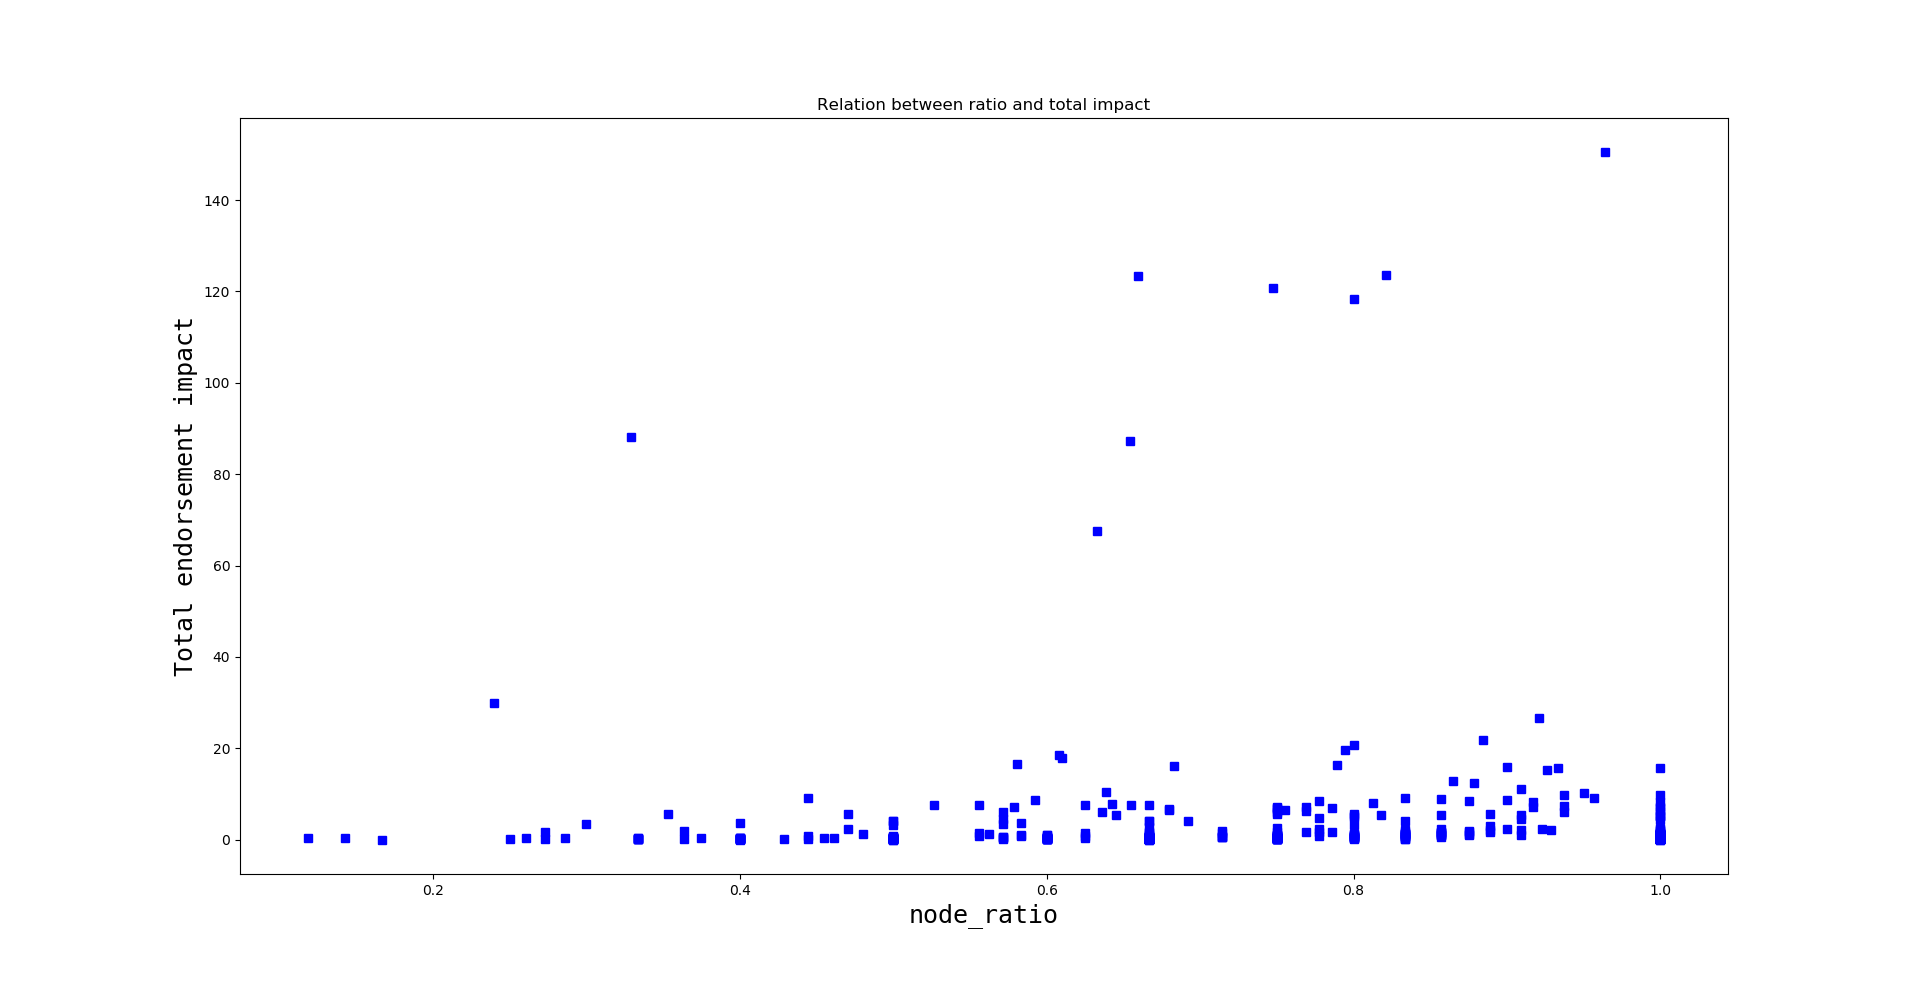
\includegraphics[width=0.95\textwidth]{Images/ratio_impact_impactAboveZero.eps}
\begin{figure}
	\includegraphics[width=0.95\textwidth]{Images/RatioVsTEIFontsize.eps}
	\caption{Relation of Ratio and Total endorsement impact}
	\label{fig:ratioimpact}
\end{figure}
\begin{figure}
	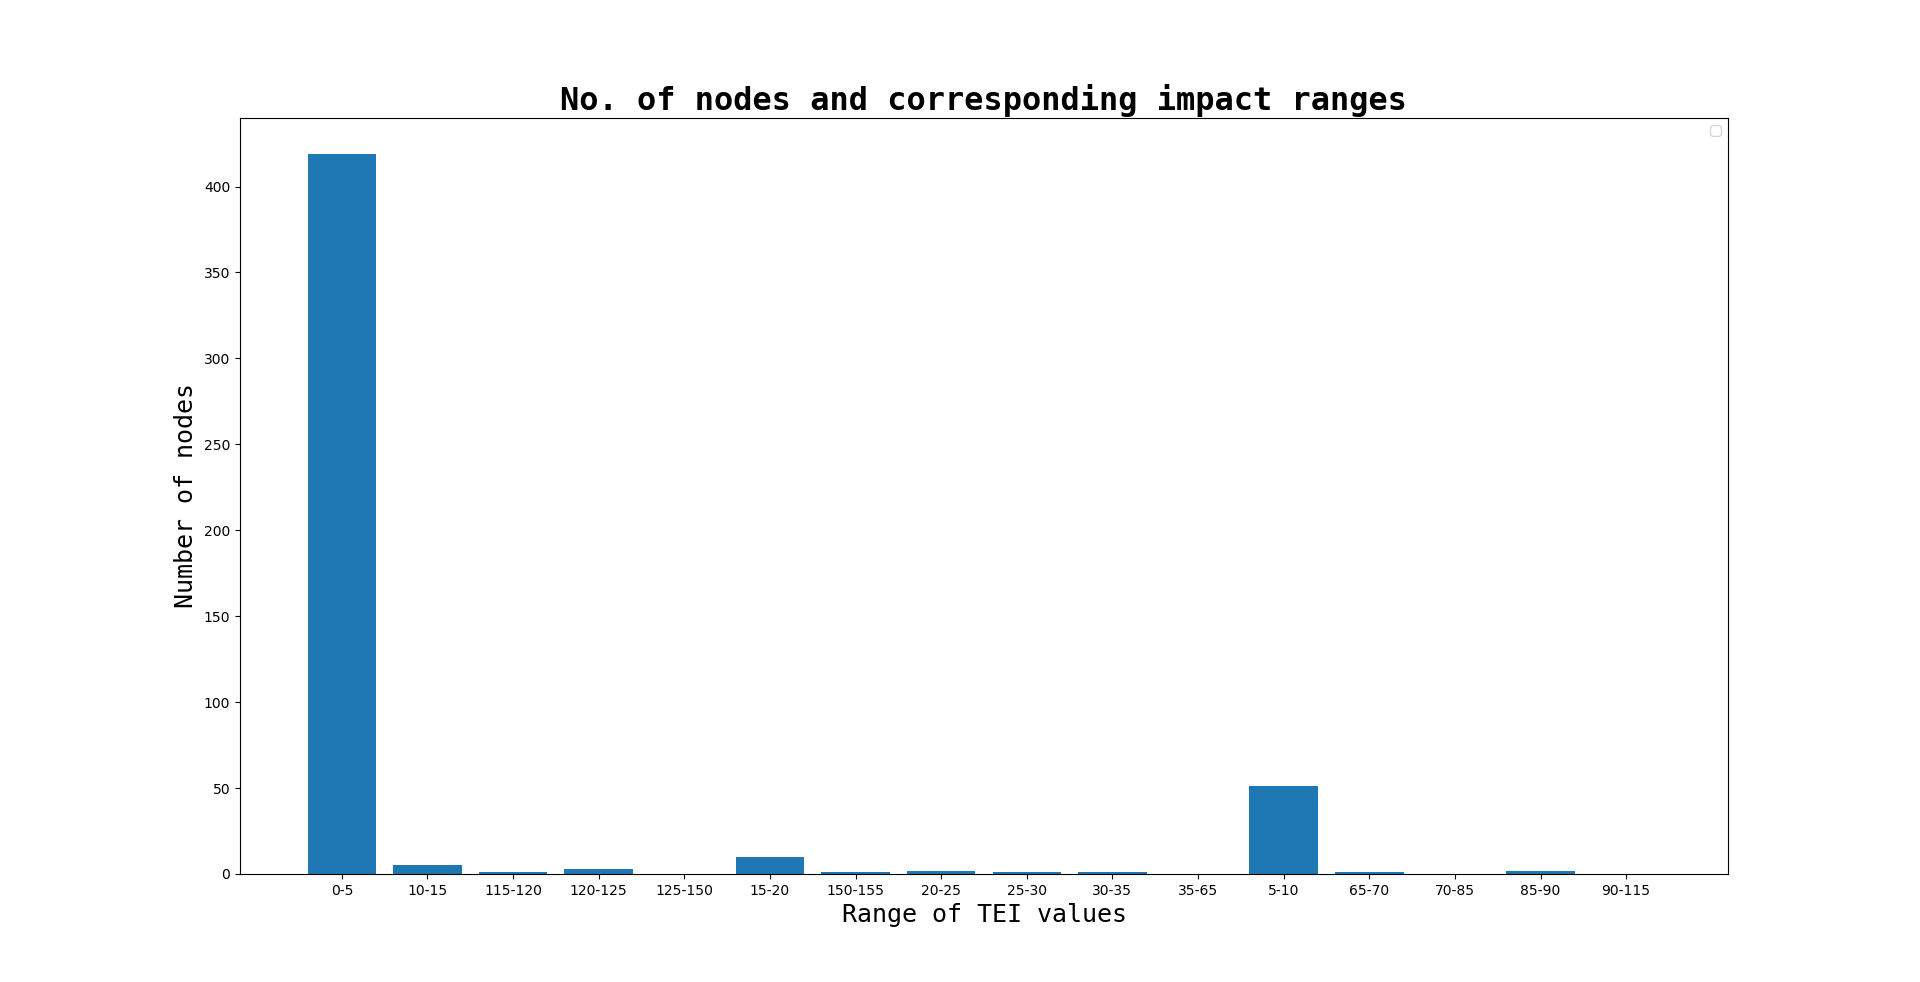
\includegraphics[width=1.0\textwidth]{Images/NoOfNodesVSImpactRanges.eps}
	\caption{Total endorsement impact vs. number of nodes}
	\label{table:totalimpact}
\end{figure}
\begin{figure}
	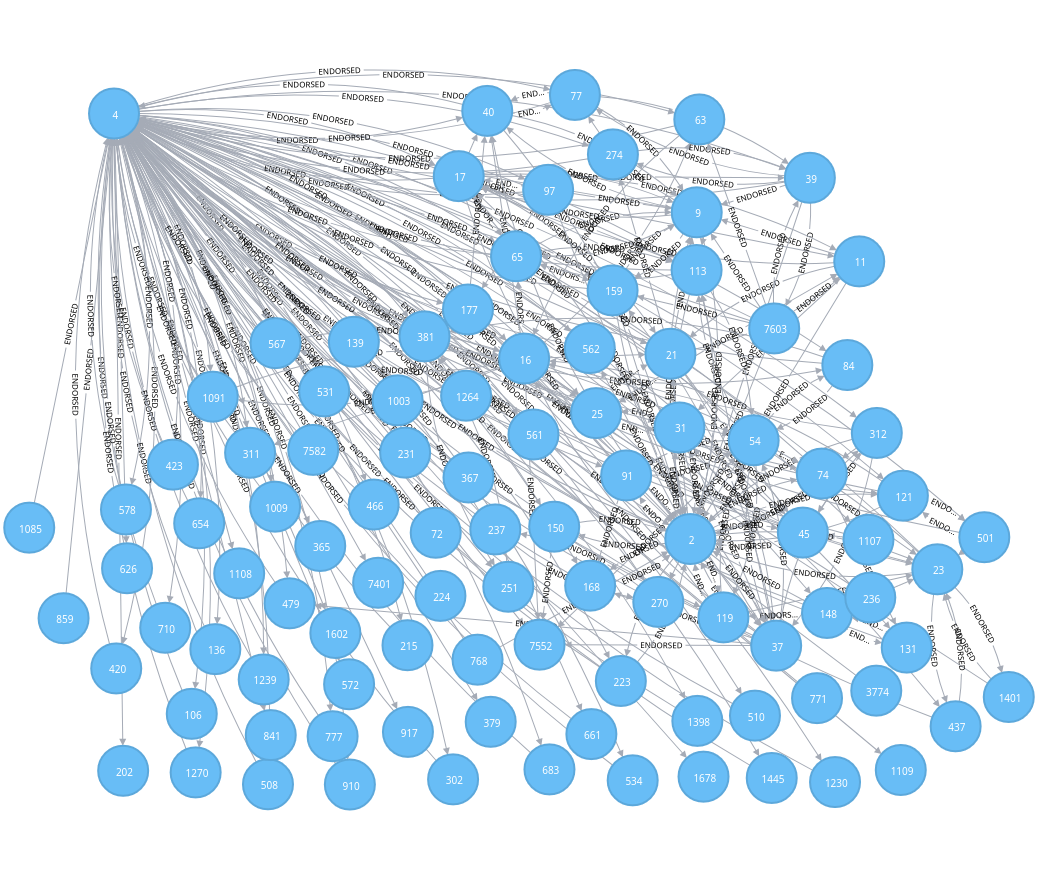
\includegraphics[width=1.0\textwidth]{Images/HighImpact_Node4.eps}
	\caption{High Impact Node}
	\label{fig:highImpactNode}
\end{figure}
%\begin{tabularx}{\textwidth}{| X | X | }
%  \hline
%   \textbf{No. of nodes} & \textbf{Impact Range} \\
%  \hline 
%  419  & 0-5  \\
%  \hline
%   51 & 5-10 \\
%  \hline
%  5 & 10-15 \\
%  \hline
%  10 & 15-20 \\
%  \hline
%  2 & 20-25 \\
%  \hline
%  1 & 25-30 \\
%  \hline
%  1 & 30-35 \\
%  \hline
%  0 & 35-65 \\
%  \hline
%  1 & 65-70 \\
%  \hline
%  0 & 70-85 \\
%  \hline
%  2 & 85-90 \\
%  \hline
%  0 & 90-115 \\
%  \hline
%  1 & 115-120 \\
%  \hline
%  3 & 120-125 \\
%  \hline
%  0 & 125-150 \\
%  \hline
%  1 & 150-155 \\
%  \hline
%  \caption{No. of nodes and the corresponding impact ranges}
%  \label{table:totalimpact}
%\end{tabularx}
\section{Total impact across several factors with different
scenarios}\label{Allcases}
This section considers different scenarios to analyze how several factors
such as \ac{nEG}, \ac{nER}, ratio, \ac{TRP} is distributed and what
contributes to having a higher or a lower \ac{TEI} value.  First two cases look
at the nodes with maximum impact value. As mentioned earlier, a node that does
not have a maintained ratio cannot have a higher impact value. As such, it is
interesting to see the minimum ratio that a maximum impact node has. Case1 and
Case 2 shows this behavior. Similarly, the third and fourth case also makes the
same analysis but with nodes having minimum impact value. The
Figure~\ref{fig:allCases} shows the distribution across several factors for all
four cases mentioned. 
\begin{figure}[h]
	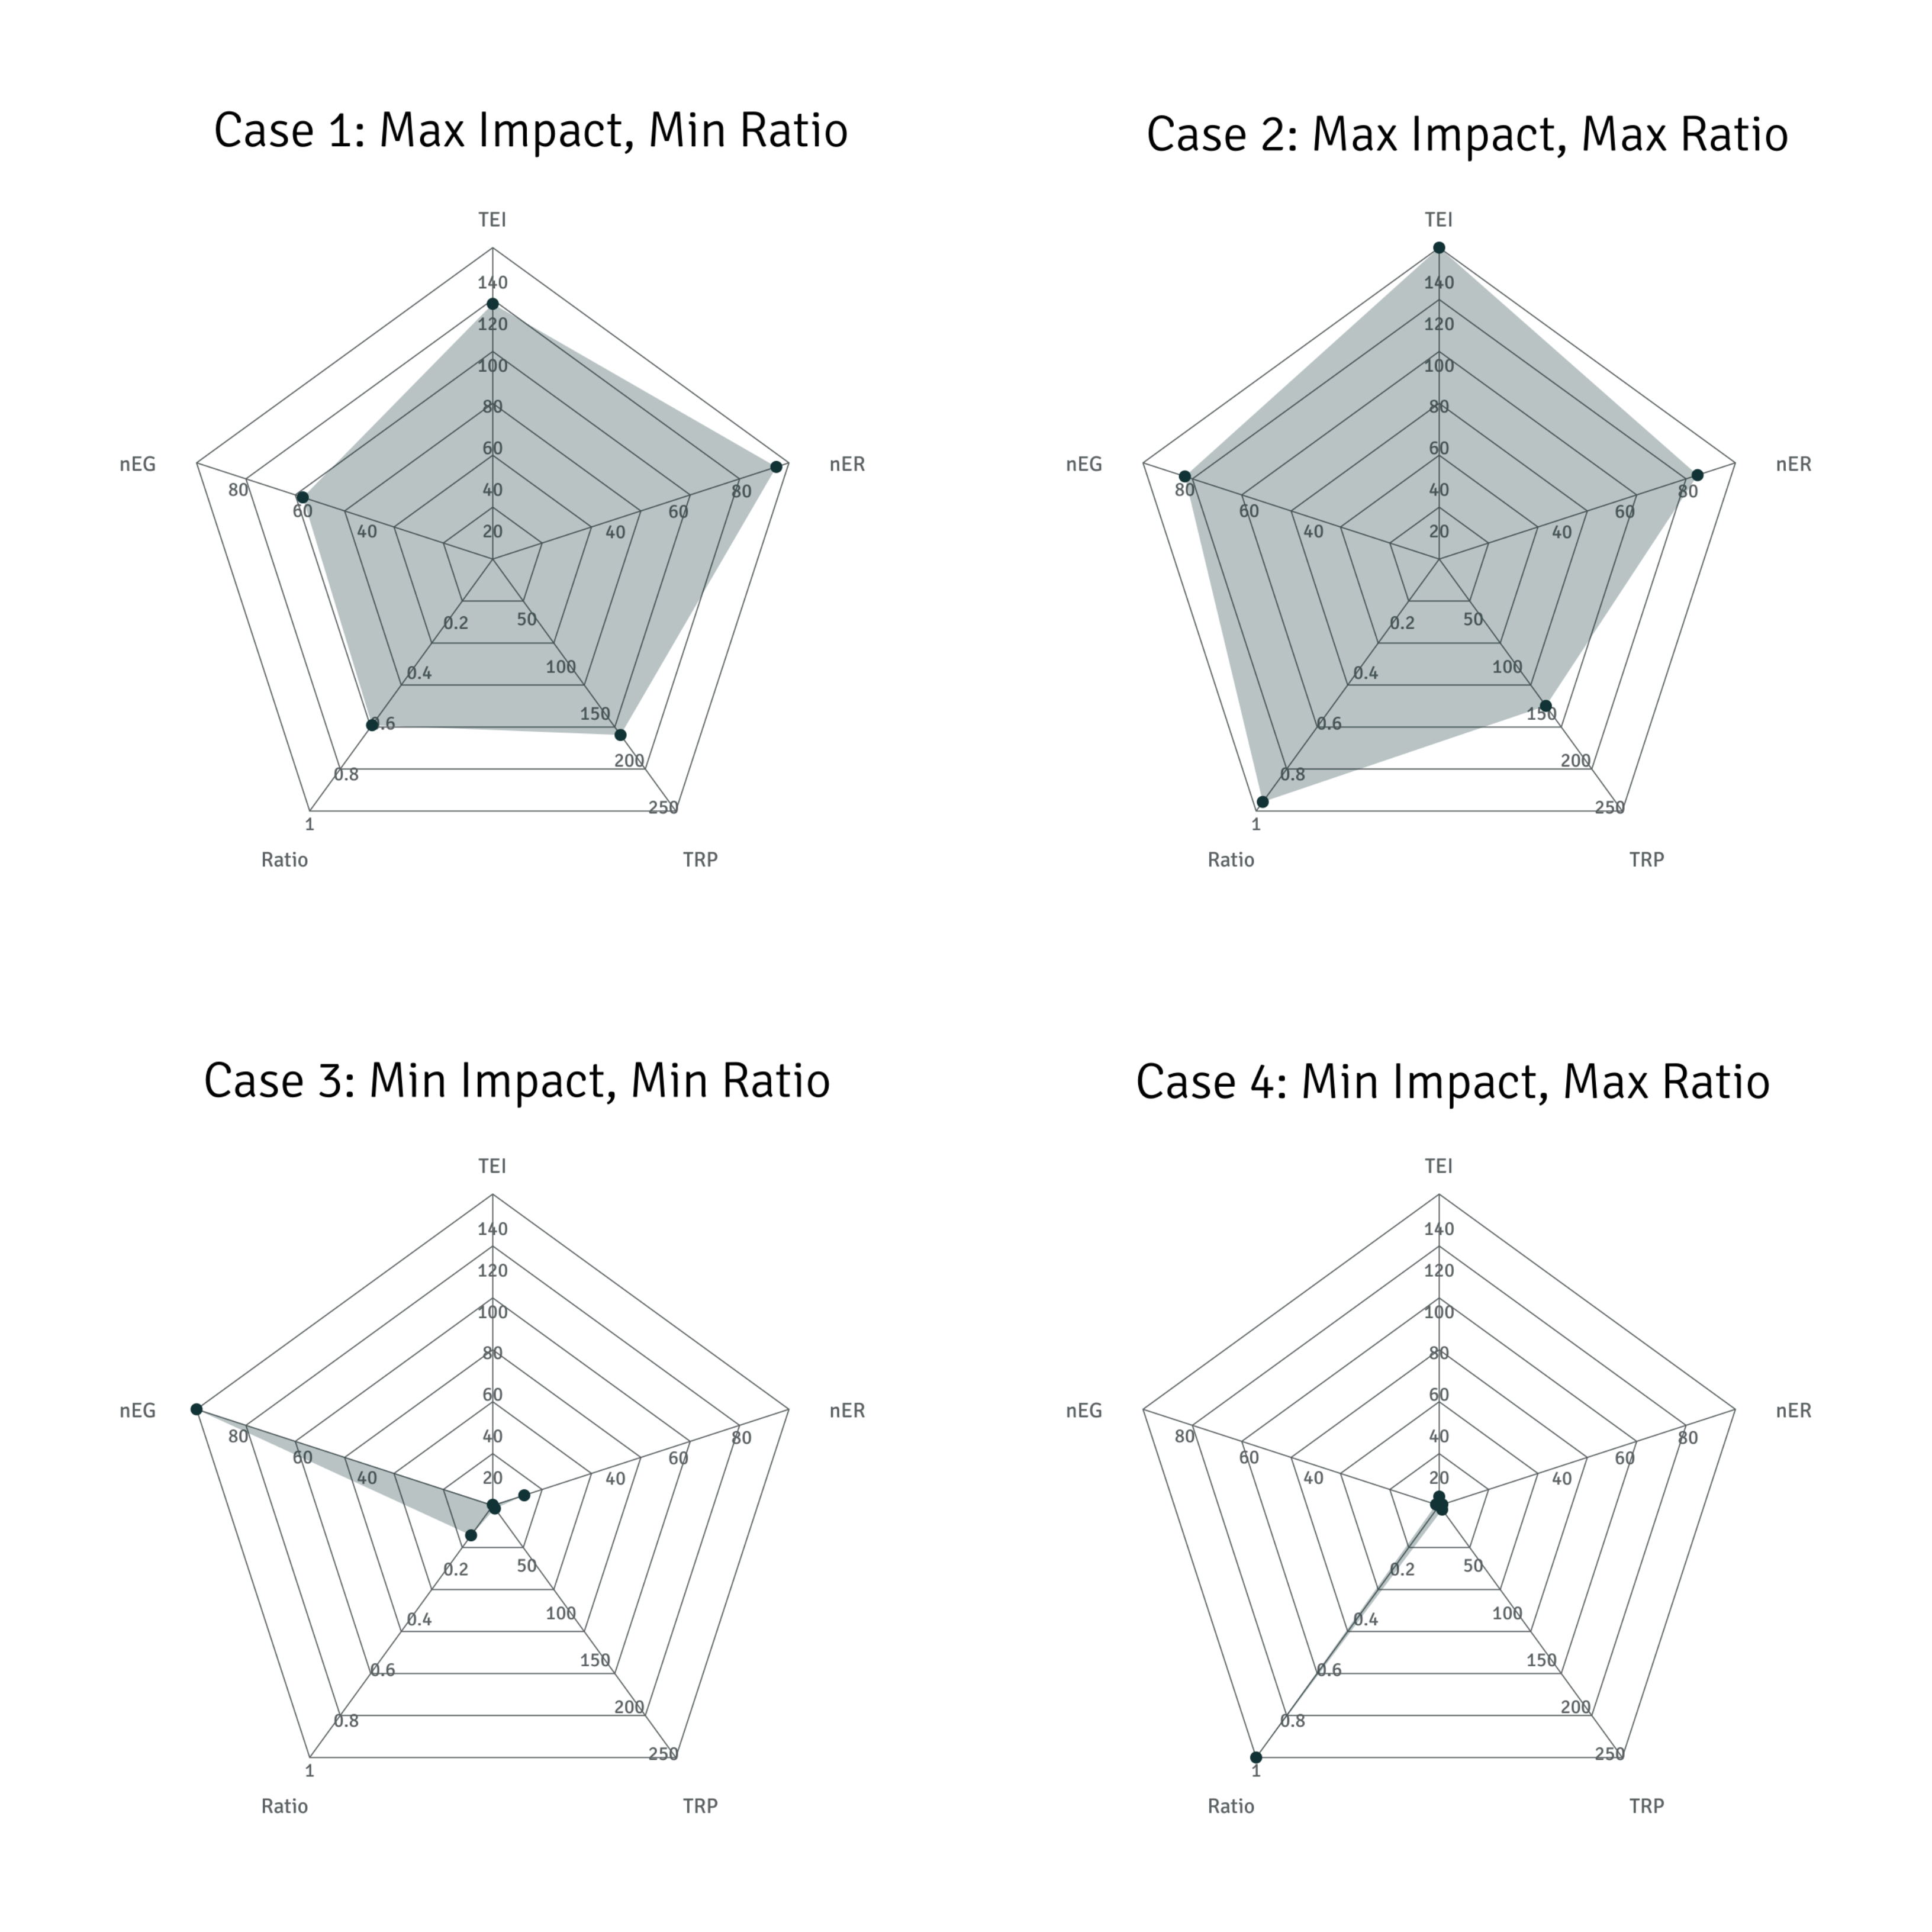
\includegraphics[width=0.9\textwidth]{Images/AllCases-acronyms.eps}
	\caption{Total Impact Across all factors}
	\label{fig:allCases}
\end{figure}
\paragraph{Case 1 \& Case 2:}The lowest ratio of the node with maximum impact
value is 0.6 and has a significant number of outgoing and incoming connections
which looks balanced as expected for a higher impact node. Similarly, the
maximum ratio that a node with the maximum impact has is 1, which is the
highest possible value. As such, the nodes with higher \ac{TEI} score
represents the honest nodes with expected interactions behavior. 
\paragraph{Case 3 \& Case4:}We can see from the Figure~\ref{fig:allCases} the
node has the lowest impact value because of an extreme one-way connection in
case 3. It has too many outgoing connections and comparatively very few
incoming connections making it evident why the node has such a low impact
value. 

\section{Threat Model}\label{sec:threatModel}
Relevant threat models and how the endorsement system addresses them is
presented in this section. 
\paragraph{Sybil attack:} The endorsement system addresses the Sybil attack by
requiring the endorsers of a peer to have a high impact value as well. A peer
can create multiple identities and self-interact to send a large number of
endorsements to direct to themselves. However, being endorsed by a new set of
endorsers (or endorsers with no activity on the network) does not help to get a
higher value as discussed earlier in Section~\ref{sec:interaction}. To overcome
this, a malicious node may try to send endorsements among each other such that
each identity has a significant impact value leading to a better trust score on
the identity they intend to inflate the score of. However, doing so requires
sending many endorsement transactions over to the etherum network and raises
the cost of operation. 
\paragraph{whitewashing:}The idea of rewards and punishment discussed in
Section~\ref{rewardpunishment} can aid in lessening a whitewashing behavior. By
punishing the misbehaving nodes in a way that decreases their score made so far
significantly but still preventing the value to be lower than a new user,
whitewashing can be addressed. The punishment of a node requires communication
with the transaction network to receive the feedback on a transactional
outcome. 
\paragraph{Freeriders:} Free riders issue is addressed by requiring the nodes
to have a balanced ratio of outgoing and incoming connections.
\paragraph{Denial of service:} Denial of service is addressed by deploying the
endorsement system on a public, permissionless blockchain network. There is no
way to know a priori the address of a validator node that will be signing the
next block. Therefore, attackers do not know where to direct the attack to
intrude the operation of endorsement transactions. 
\paragraph{Self-promoting and Slandering attack:}The cryptographic functions of
the blockchain solve the possibility of this attack due to lack of data source
authentication or data integrity verification, and once the transaction is
added to the blockchain, the blockchain protocol provides the guarantee of the
immutability of data and offers public verifiability of data. Another reason
this attack is possible is by creating multiple Sybil identities. The Sybil
attack has been discussed earlier. 
\paragraph{Malicious collective:}Malicious nodes can form a collective group
and endorse each other until they all have a high \ac{TEI} value to be
considered trustworthy in the endorsement network. The endorsement system
metrics allow the possibility for malicious collectives to be seen as more
trustworthy. The current implementation of the endorsement system does not
address this issue. However, the information available about an entity can be
used, if needed to find out malicious nodes that explicitly interact within
their group. \par
Consider a malicious collective of four nodes, $M = \{A,B,C,D\}$ that endorses
each other. The endorsement system maintains two sets of data for each
participant, one that contains the list of endorsers, and other that contains
the list of endorsees. \par
If $A$ represents the list of endorsers and $A'$ represents the list of
endorsees for the entity $A$, then, we can find the intersection of the sets
$A$ and $A'$ to find out the list of common entities in these two sets. The
elements of this intersection set should represent the entities with whom $A$
has the symmetric trust relation with.  
\begin{equation}
	\begin{split}
	A= \{B,C,D\} \\
	A' = \{B,C,D\} \\
	A \cap A' = \{B,C,D\}
\end{split}
\end{equation}
As we can see that the intersection set includes the same list as the list of
endorsers and endorsees, it is most likely that these entities are forming a
malicious collective to inflate each other's trust scores. However, this does
not provide enough information to infer that a node is malicious with
certainty. We cannot ignore the possibility that they know each other and the
endorsement interaction is an honest one. The characteristic of trust as being
asymmetric does not invalidate the existence of the symmetric trust, i.e., $A$
trusts $B$ does not imply $B$ has to trust $A$ but it is entirely up to $B$ if
he trusts $A$, and only $B$ knows if the trust relationship is an honest or
malicious one. \par
Hoffman K, Zage D, Nita-Rotaru C~\cite{hoffman2009survey} relates the process
of finding the colluding nodes as such to finding a clique~\footnote{A
clique~\cite{cormen2009introduction} in an undirected graph $G = ( V,E)$ is a
subset $V' \subseteq V$ of vertices, each pair of which is connected by an
edge in $E$.} of a certain size in a graph, which has been known to be
NP-complete and only has heuristic based solutions.  An important consideration
to be taken if one wants to find the intersection of sets of endorsers and
endorsees is that as the size of the sets grows, so does the computational
complexity. Given, the amount of gas that each operation costs, it does not
seem to be a feasible solution for doing this form of computation on ethereum
blockchain. As such, it is recommended to implement it on a client-side and
only make the computation if invoked by the client.

%\section{Summary of Results}

%\section{Blockchain: Gas Consumption, Block size, Transactions}
%Ethereum  specific concepts:
%As mentioned earlier, executing any operation on Ethereum costs some amount of
%gas. The total amount of transactions that can be included in an Ethereum block
%is therefore not determined by the size but by the amount of gas consumed by
%them. The block limitation is about 4 million gas per block.  The current block
%according to etherscan\footnote{http://etherscan.io/} is Block number 5778648
%with a total of 155 transactions recorded in it. The time between the previous
%block and the current block is around 11 seconds. Thus, the network throughput
%based on this data is around 11 transaction per second. The average block time is 17 seconds which is dynamically adjusted based on how fast or slow 
%





%The gas consumption for the transactions in endorsement contract is based on
%the tests performed on Rinkeby test network and remix environment. The gas
%price and gas limit are based on the statistics from the main ethereum network
%\footnote{https://ethgasstation.info/index.php}. The gas cost to join the
%endorsement network is 142927 units of gas and to send an endorsement is 203746
%units of gas. Recommended safe low value for the gas price is 2
%Gwei(0.000000002 eth). 
%The block size limitation in ethereum is about 4 million gas per block.
%Therefore, the total amount of transactions is not determined by its size but
%by the amount of gas it consumes. The current block according to
%etherscan\footnote{http://etherscan.io/} is Block number 5778648 with a total
%of 155 transactions recorded in it. The time between the previous block and the
%current block is around 11 seconds. Thus, the network throughput based on this
%data is around 11 transaction per second. 










%\section{Analysis}
%\section{Measurement}
%\section{Comparison}

% Presentation of results and case-study data 
% An application of the methodology is unfolded and results are presented using for example via Charts, Diagrams, Figures and Tables 
% The work is conducted in accordance with the method described earlier. Results are presented in an analytical way.
